\documentclass[10pt]{article}
\usepackage[a4paper,margin=18mm]{geometry}
\usepackage[T1]{fontenc}
\usepackage{lmodern,graphicx,amsmath,amssymb,booktabs,xcolor,hyperref}
\hypersetup{colorlinks=true,urlcolor=blue,linkcolor=blue}
\setlength{\parindent}{0pt}\setlength{\parskip}{4pt}
\begin{document}
{\Large Curve25519 section coefficients: reduced support, growing degree}\par
2026-11-23\quad PR4984\quad Native source\texttt{112d723022}\par
\textbf{Standing: producer unsigned/unverified.} Native PCC-ddf583;
written conditional derivation PCC-eae0ef.

The Rust component qualifies a simpler supplied-coefficient predicate for the
original distinct-raw-column torus base. The five coefficients remain supplied.
The reduction concerns valid $\mathbb F_p$ assignments, not arbitrary
algebraic-closure solutions or a coefficient-discovery algorithm.

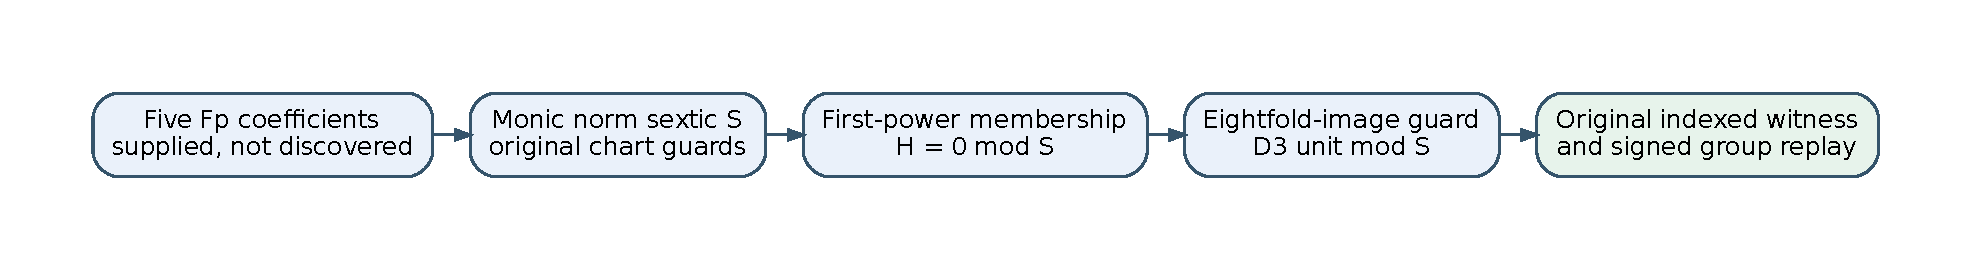
\includegraphics[width=\linewidth]{flow.pdf}

For $R=(r,s)$, $s\ne0$, normalize $c_4=1$ and write
\[
 U=(X-r)(c_0+c_1X+c_3X^2)+c_5s,\qquad
 V=(X-r)(c_2+X)+c_5,
\]
\[
 S=-\frac{U^2-(X^3+AX^2+X)V^2}{X-r}.
\]
This monic sextic has five free field inputs. The identity-$R$ chart instead
normalizes $c_5=1$. Finite two-torsion targets remain unsupported.

\textbf{Reduced support.}
For odd exact torus order $aq$, $2k<a$, the signed-trace polynomial
$H_\lambda(T)=\prod_{j=1}^k(T_q(T)^2-\Re(h^{qj})^2)$ has $D=2qk$ distinct
displayed roots $\pm\Re(h^{j+at})$ in $\mathbb F_p$. Its cleared Moebius
pullback $E_B$ is split and squarefree. The trace/inversion argument also
makes raw pre-image $x$ injective on the positive window, while repeated
eightfold images remain legal.

If $S\mid E_B$, nonsquare $C(x)$ would force $U(x)=V(x)=0$, hence a double
factor of $S$ away from the forced target factor. At the target its ordinate
is already rational. Membership excludes zero ordinates. Thus, under the
written norm/chart hypotheses, explicit Frobenius and ordinate tests can be
replaced by
\[
 E_B\bmod S=0,\qquad \gcd(S,D_3)=1.
\]
Here $D_3$ is the denominator after three classical Montgomery XZ doublings;
the unit guard removes identity eightfold images. The original map-inverse
guard and complete indexed witness/group replay stay. Full exceptional-case
argument: \path{section-coeff-v1/DERIVATION.md}.

\textbf{Fixed native qualification.}\par
\begin{tabular}{p{10.5cm}r}
\toprule
Control & Observation\\\midrule
Toy raw columns / distinct signed-trace map roots &24 / 48\\
Supported original replays / unsupported two-torsion charts &1770 / 22\\
Declared six-column signed tuples / supported identity-$R$ cases &1792 / 16\\
101 coefficient values: replay / predicate refusal / map refusal &1 / 98 / 2\\
Exact formal-degree pencils &8 / 8\\
Original actual-field supplied sections, $k=31,20633$ &2 / 2\\\bottomrule
\end{tabular}

One frozen worker completes1810 records including completion. Repeated raw
support passes old sixth-power membership but fails first power; a distinct
support containing an identity image fails the $D_3$ unit test. Actual controls
retain $q=213156431$, $a=60824497$ and extract $j=1,\ldots,6$, $t=0$.
No target cohort, actual-base enumeration or coefficient discovery is implied.
The dense toy polynomial is built from the displayed raw roots; fast versus
dense comparison covers the101 coefficient-pencil values. References share
field primitives, rather than independently implementing every bridge.

\newpage
{\large Degree audit and the next scaling obligation}\par
On the formal pencil $c_3=T$, $s_5=-T^2+\text{lower terms}$. In reducing the
leading $X^D$ term modulo monic $S$, only the repeated $-s_5$ path drops one
$X$ degree for every two $T$ degrees. All other paths have strictly smaller
$T$ degree. Lower terms of $E_B$ cannot cancel this leading path. Therefore
the literal $X^5$ remainder coefficient has exact formal degree
\[
 2(D-5)=4qk-10.
\]
The eight native pencils evaluate exact polynomials in $\mathbb F_{101}[T]$,
without reduction by $T^{101}-T$. The actual integer formula gives
$17{,}592{,}226{,}563{,}282$; the actual polynomial is never expanded.

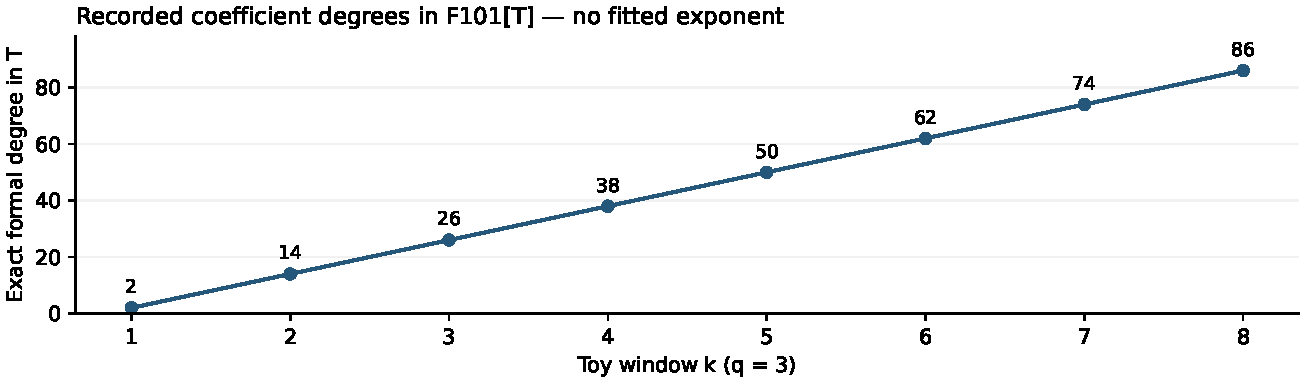
\includegraphics[width=\linewidth]{degree.pdf}

\textbf{Interpretation.}
This literal encoding does not have degree bounded independently of the base.
Its degree is not a lower bound on solving degree, regularity, minimal
generators or another solver. Five inputs and small evaluation circuits alone
do not supply a root-finding complexity bound. Generic RR9 radical support,
Chebyshev trace laws, norms and XZ doubling are prior art; no novelty clearance
or algorithmic speed claim is made.

\textbf{Next technical step.}
Compile unknown coefficients through the guarded first-power arithmetic
circuit, then establish extension/projection for $\mathbb F_p$ assignments
and a structured elimination/root-extraction work bound. Charge field-bit
costs, setup, failed attempts, memory, original indexing/lifting and useful
rank under the original family, private selection, kernel and recovery contract.
Avoid all-triple construction. No solver campaign or empirical exponent fit
is scheduled by this component report.

\textbf{Formal scope.}
Two existing-law endpoints over $\mathrm{ZMod}(2^{255}-19)$ pass the maintained
file audit: squarefree inheritance (PCC-548372) and no squared linear divisor
(PCC-aa408d). They use standard axioms only,2 named theorems/0 failing/0
trusted native. Trace splitting, norm/line-bundle binding, ordinate rationality,
native/group refinement and the degree induction remain unformalized. The
local audit is not signed standing. \path{PROOF_MAP.md} states the exact scope.

\textbf{Provenance and reproduction.}
The41-input closure combines the unchanged30-input58112-byte v1 archive and
an11-input13500-byte delta. Eight compiled hashes and the1651728-byte copied
binary\texttt{19a02061785d} match pre/post; four focused release tests,fmt and
strict Clippy pass. Separately copied immutable qualifier, create-new raw
output, distinct BUILD/PRECALL/POSTCALL and actual transport collision are
retained. The4581082-byte JSONL\texttt{7b59c8519927} is complete inside the
164272-byte native archive\texttt{8f7b6024a389}. Its trusted store receipt
is a separate publication gate; see\path{PUBLISHING.md}. No timing, RSS,
complete bitop or independent execution receipt is inferred.

\textbf{Primary sources.}
\href{https://arxiv.org/abs/1209.4396}{Gassert, arXiv1209.4396}
(monic trace normalization scaled to half-trace);
\href{https://hyperelliptic.org/EFD/g1p/auto-montgom-xz.html}{EFD Montgomery XZ};
\href{https://doc.sagemath.org/html/en/reference/arithmetic_curves/sage/schemes/hyperelliptic_curves/jacobian_morphism.html}{official Sage Mumford documentation}.
Internal RR9 radical-support result and frozen v1 norm/extraction contracts
are retained. KB unavailable; Cantor1987 AMS primary PDF403.
\end{document}
